\documentclass{scrartcl}

\reversemarginpar
\newcommand{\MarginDate}[1]{\marginpar{\raggedleft\itshape\small#1}}
\usepackage[utf8]{inputenc}
\usepackage[T1]{fontenc}
\usepackage[LabelsAligned]{currvita}
\usepackage[nochapters]{classicthesis}
\usepackage{url}
\renewcommand{\cvheadingfont}{\LARGE\color{Maroon}}
\renewcommand{\cvlistheadingfont}{\large}
\renewcommand{\cvlabelfont}{\qquad}

\usepackage{hyperref}		
\hypersetup{	colorlinks,breaklinks,
			urlcolor=Maroon, 
			linkcolor=Maroon}
\usepackage{eurosym}
\newlength{\datebox}\settowidth{\datebox}{\small{2008.02 $\rightarrow$ 2009.04}}

\newcommand{\NewWorkExperience}[3]{\noindent\hangindent=2em\hangafter=0 \parbox{\datebox}{\textit{#1}}\hspace{1.5em} #2 #3%
\vspace{0.5em}}

\newcommand{\Description}[1]{\hangindent=2em\hangafter=0\noindent\raggedright\footnotesize{#1}\par\normalsize}
\newcommand{\Sep}{\vspace{2em}}

\usepackage{textpos}
\usepackage{graphicx}

\setlength{\TPHorizModule}{10pt}
\setlength{\TPVertModule}{10pt}



\usepackage[left=4.5cm, right=2.5cm, top=1.5cm, bottom=2.5cm]{geometry}



\begin{document}
\thispagestyle{empty}
\begin{cv}{\spacedallcaps{Remus Mihail Prunescu}}
\vspace{1.5em}

\begin{textblock}{1}(-10,0) %
\frame{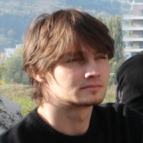
\includegraphics[scale=0.5]{rprunescu.png}}
\end{textblock}


\noindent\spacedlowsmallcaps{Personal Data}
\vspace{0.5em}

\NewWorkExperience{}{\textit{Born in Romania,}}{29 December 1984}

\NewWorkExperience{email}{\href{mailto:remusmp@protonmail.com}{remusmp@protonmail.com}}{}

\NewWorkExperience{phone}{+45 53 77 55 84}{}

\NewWorkExperience{www}{\href{http://remusmp.github.io/}{remusmp.github.io}}{}
\vspace{1.5em}





\noindent\spacedlowsmallcaps{Work Experience}
\vspace{0.5em}

\NewWorkExperience{\small{2016.01 $\rightarrow$ Now}}{Propeller Control}{- Copenhagen, Denmark}

\Description{\MarginDate{Development Engineer (R\&D)\\[1em]{\normalfont{\tiny Real-Time Hardware\\ C/C++\\python\\git\\}}}%
\textbf{Description:} Advanced control algorithms for the maritime industry.
\begin{itemize}
    \item Model-based design and testing of a new engine power controller;
    \item A C/C++ numerical library for filtering, state estimation and model predictive control (MPC);
    \item A very fast implementation of a complex closed loop that takes 3ms to execute on the real-time hardware;
    \item Extensive data analysis to assess the control performance.
\end{itemize}
}

\Sep

\NewWorkExperience{\small{2012.04 $\rightarrow$ 2016.01}}{\href{www.dongenergy.com}{DONG Energy}}{- Copenhagen, Denmark}

\Description{\MarginDate{Industrial PhD Student (R\&D)\\[1em]{\normalfont{\tiny Dynamic Modelling\\Nonlinear Systems\\Control Theory\\Process Optimization\\C/C++\\Matlab/Simulink\\python\\git\\}}}%
\textbf{Project:} Dynamic Modeling, Optimization and Advanced Control for Large Scale Lignocellulosic Biorefineries.
\begin{itemize}
    \item Modeling and validation of a dynamic simulator for large scale plants;
    \item All my work includes uncertainty and sensitivity analysis, aspects often overlooked by other researchers;
    \item Process optimization at a large scale that maximizes the refinery profit;
    \item Peer-reviewed contributions listed on my \href{http://remusmp.github.io}{website}.
\end{itemize}
}

\Sep

\NewWorkExperience{\small{2009.11 $\rightarrow$ 2015.10}}{\href{www.dtu.dk}{Technical University of Denmark}}{- Kgs. Lyngby}
\Description{\MarginDate{\LaTeX\ Supporter}%
\begin{itemize}
    \item Teaching and offering support to other students developed my soft skills such as: training, public speaking, listening and supervision;
    \item Contributed with templates for slide shows, PhD and MSc thesis, and course reports.
\end{itemize}}


\Sep

\NewWorkExperience{\small{2008.08 $\rightarrow$ 2009.03}}{\href{www.bitdefender.com}{BitDefender}}{- Bucharest, Romania}

\Description{\MarginDate{Software Developer\\[1em]{\tiny C/C++\\ Multithreading\\gtest}}%
\textbf{Description:} BitDefender is a successful security software company. I was a member of the Desktop team, which had as objective the integration of the security tools into a user friendly application ready to be shipped to end users. Achievements: 
\begin{itemize}
    \item Introduced the team to new unit testing frameworks;
    \item Wrote the first unit tests in \href{https://github.com/google/googletest}{gtest}.
\end{itemize}
}

\Sep

\NewWorkExperience{\small{2006.06 $\rightarrow$ 2007.09}}{\href{http://www.ama-studios.com/}{AMA}}{- Bucharest, Romania}

\Description{\MarginDate{Software Developer}%
\textbf{Description:} AMA or Advanced Mobile Applications is a social software developer for mobile devices. Achievements:
\begin{itemize}
    \item Optimize code to run on devices with limited resources (small memory and slow CPU);
    \item Rewrote parts of the API to make them more efficient.
\end{itemize}}


\vspace{1.5em}

\noindent\spacedlowsmallcaps{Education}
\vspace{0.5em}

\NewWorkExperience{\small{2012.04 $\rightarrow$ 2015.11}}{\href{http://orbit.dtu.dk/en/persons/remus-mihail-prunescu\%28f26a9ff8-23c2-4cb4-a93d-43135e6afbb6\%29.html}{Industrial PhD Student}}{}

\Description{\MarginDate{Technical University of Denmark}%
\textbf{Thesis title:} Dynamic Modeling, Optimization, and Advanced Control for Large Scale Biorefineries.\\
See my work experience as an industrial PhD student at DONG Energy.}

\Sep

\NewWorkExperience{\small{2009.08 $\rightarrow$ 2011.10}}{MSc. in Automation and Robot Technology}{}

\Description{\MarginDate{Technical University of Denmark}%
\textbf{Thesis title:} Thermal Reactor Modeling and Control for Bio-Ethanol Production Processes. This research deals with modeling and control of a thermal reactor for biomass pretreatment using computational fluid dynamics tools.\newline
\textbf{GPA: 10.7/12}}


\Sep

\NewWorkExperience{\small{2004.09 $\rightarrow$ 2009.06}}{Engineer Diploma in Automatic Control}{}

\Description{\MarginDate{University Politehnica, Bucharest, Romania}Courses oriented towards automation and software engineering. I wrote my diploma thesis as an exchange student at Université de Picardie Jules Verne (UPJV) in Amiens, France. The paper was entitled \textbf{Vehicle Dynamics and Control} and it approaches new vehicle control techniques meant to improve the stability and the maneuverability of a 4 wheel steering machine.\newline
\textbf{GPA: 9.2/10}}


\vspace{1.5em}
\spacedlowsmallcaps{Additional Information}
\vspace{0.5em}

\NewWorkExperience{}{\hspace{-9.38em}Honors and Awards}{}

\Description{Speaker and Chair of Biofuel Session, World Congress of Chemical Engineering 9 (August 2013), Seoul, South Korea. \textbf{Advances in Monitoring, Diagnosis and Control of Biorefineries}.}
\vspace{0.5em}
\Description{Best Presentation in Session Award, The American Control Conference 2013, Washington D.C., USA. \textbf{Modeling and L1 Adaptive Control of pH in Bioethanol Enzymatic Process}.}



\Sep
\NewWorkExperience{}{\hspace{-9.38em}Publications}{}

\Description{\MarginDate{\color{black}PhD Thesis}Prunescu R. M., 2015. \href{http://orbit.dtu.dk/files/123437594/Remus_phdthesis.pdf}{Dynamic Modeling, Optimization and Advanced Control for Large Scale Biorefineries}.}
\vspace{0.5em}

\Description{\MarginDate{\color{black}Journal Papers}Prunescu R. M., Sin G., Blanke M., J. G. Jakobsen, 2015. \href{http://onlinelibrary.wiley.com/doi/10.1002/aic.14954/abstract}{Dynamic modeling and validation of a biomass hydrothermal pretreatment process - A demonstration scale study.} AIChE Journal, vol. 61, p. 4235-4250.}
\vspace{0.5em}
\Description{Prunescu R. M., Sin G., 2013. \href{http://dx.doi.org/10.1016/j.biortech.2013.10.029}{Dynamic modeling and validation of a lignocellulosic enzymatic hydrolysis process - A demonstration scale study.} Bioresource Technology, vol. 150, p. 393-403.}


\Sep






\NewWorkExperience{}{\hspace{-9.38em}Language Skills}{}

\newlength{\langbox}
\settowidth{\langbox}{Romanian}
\Description{\parbox{\langbox}{\textsc{English}}\ \ $\cdotp$\ \  \ Fluent \hspace{3.53cm} \parbox{\langbox}{\textsc{Danish}}\ \ $\cdotp$\ \  \ Beginner}
\MarginDate{Languages}

\Description{\parbox{\langbox}{\textsc{French}}\ \ $\cdotp$\ \  \ Advanced \hspace{3cm} \parbox{\langbox}{\textsc{Romanian}}\ \ $\cdotp$\ \ \  Mother Tongue}

\Sep


\NewWorkExperience{}{\hspace{-9.38em}Computer Skills}{}

\Description{\MarginDate{Engineering Tools}Matlab/Octave (Expert), Simulink (Expert)}

\vspace{0.5em}
\Description{\MarginDate{Programming}C/C++ (Expert), \LaTeX\ (Expert), Python (Advanced)}

\vspace{0.5em}
\Description{\MarginDate{Databases}SQL (Advanced), sqlite, HDF5}



\Sep
\NewWorkExperience{}{\hspace{-9.38em}Hobbies}{}

\Description{\MarginDate{Sports}Half marathon runner. I also play futsal for a local club in the Copenhagen Futsal league.}
\vspace*{-0.5em}
\end{cv}
\end{document}